\documentclass{article}

\usepackage[lmargin=1in, rmargin=1in]{geometry}
\usepackage{amsmath, amssymb, amsthm}
\usepackage{lmodern}
\usepackage{tikz}
\usepackage{pgfplots}
\usepackage{color}
\begin{document}
\begin{figure}
\centering
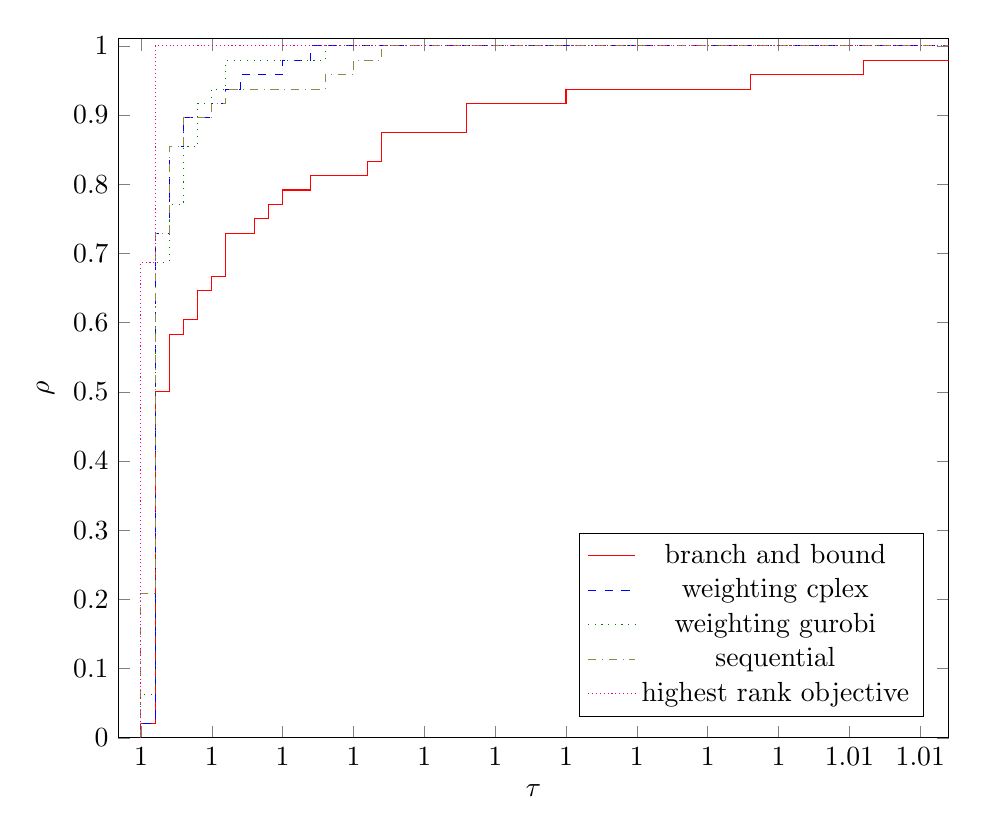
\begin{tikzpicture}
\begin{axis}[legend pos=south east, xmin=0.999840682658, xmax=1.0057, ymin=0, ymax=1.01, width=\textwidth, xlabel=$\tau$, ylabel=$\rho$, 
]
\addplot[const plot, mark=none, red, solid]
coordinates
{
(1,0)
(1, 0.0208333333333)
(1.0001, 0.5)
(1.0002, 0.583333333333)
(1.0003, 0.604166666667)
(1.0004, 0.645833333333)
(1.0005, 0.666666666667)
(1.0006, 0.729166666667)
(1.0007, 0.729166666667)
(1.0008, 0.75)
(1.0009, 0.770833333333)
(1.001, 0.791666666667)
(1.0011, 0.791666666667)
(1.0012, 0.8125)
(1.0013, 0.8125)
(1.0014, 0.8125)
(1.0015, 0.8125)
(1.0016, 0.833333333333)
(1.0017, 0.875)
(1.0018, 0.875)
(1.0019, 0.875)
(1.002, 0.875)
(1.0021, 0.875)
(1.0022, 0.875)
(1.0023, 0.916666666667)
(1.0024, 0.916666666667)
(1.0025, 0.916666666667)
(1.0026, 0.916666666667)
(1.0027, 0.916666666667)
(1.0028, 0.916666666667)
(1.0029, 0.916666666667)
(1.003, 0.9375)
(1.0031, 0.9375)
(1.0032, 0.9375)
(1.0033, 0.9375)
(1.0034, 0.9375)
(1.0035, 0.9375)
(1.0036, 0.9375)
(1.0037, 0.9375)
(1.0038, 0.9375)
(1.0039, 0.9375)
(1.004, 0.9375)
(1.0041, 0.9375)
(1.0042, 0.9375)
(1.0043, 0.958333333333)
(1.0044, 0.958333333333)
(1.0045, 0.958333333333)
(1.0046, 0.958333333333)
(1.0047, 0.958333333333)
(1.0048, 0.958333333333)
(1.0049, 0.958333333333)
(1.005, 0.958333333333)
(1.0051, 0.979166666667)
(1.0052, 0.979166666667)
(1.0053, 0.979166666667)
(1.0054, 0.979166666667)
(1.0055, 0.979166666667)
(1.0056, 0.979166666667)
(1.0057, 0.979166666667)
};
\addlegendentry{branch and bound}
\addplot[const plot, mark=none, blue, dashed]
coordinates
{
(1,0)
(1, 0.0208333333333)
(1.0001, 0.729166666667)
(1.0002, 0.854166666667)
(1.0003, 0.895833333333)
(1.0004, 0.895833333333)
(1.0005, 0.916666666667)
(1.0006, 0.9375)
(1.0007, 0.958333333333)
(1.0008, 0.958333333333)
(1.0009, 0.958333333333)
(1.001, 0.979166666667)
(1.0011, 0.979166666667)
(1.0012, 1.0)
(1.0013, 1.0)
(1.0014, 1.0)
(1.0015, 1.0)
(1.0016, 1.0)
(1.0017, 1.0)
(1.0018, 1.0)
(1.0019, 1.0)
(1.002, 1.0)
(1.0021, 1.0)
(1.0022, 1.0)
(1.0023, 1.0)
(1.0024, 1.0)
(1.0025, 1.0)
(1.0026, 1.0)
(1.0027, 1.0)
(1.0028, 1.0)
(1.0029, 1.0)
(1.003, 1.0)
(1.0031, 1.0)
(1.0032, 1.0)
(1.0033, 1.0)
(1.0034, 1.0)
(1.0035, 1.0)
(1.0036, 1.0)
(1.0037, 1.0)
(1.0038, 1.0)
(1.0039, 1.0)
(1.004, 1.0)
(1.0041, 1.0)
(1.0042, 1.0)
(1.0043, 1.0)
(1.0044, 1.0)
(1.0045, 1.0)
(1.0046, 1.0)
(1.0047, 1.0)
(1.0048, 1.0)
(1.0049, 1.0)
(1.005, 1.0)
(1.0051, 1.0)
(1.0052, 1.0)
(1.0053, 1.0)
(1.0054, 1.0)
(1.0055, 1.0)
(1.0056, 1.0)
(1.0057, 1.0)
};
\addlegendentry{weighting cplex}
\addplot[const plot, mark=none, green!50!black, dotted]
coordinates
{
(1,0)
(1, 0.0625)
(1.0001, 0.6875)
(1.0002, 0.770833333333)
(1.0003, 0.854166666667)
(1.0004, 0.916666666667)
(1.0005, 0.9375)
(1.0006, 0.979166666667)
(1.0007, 0.979166666667)
(1.0008, 0.979166666667)
(1.0009, 0.979166666667)
(1.001, 0.979166666667)
(1.0011, 0.979166666667)
(1.0012, 0.979166666667)
(1.0013, 1.0)
(1.0014, 1.0)
(1.0015, 1.0)
(1.0016, 1.0)
(1.0017, 1.0)
(1.0018, 1.0)
(1.0019, 1.0)
(1.002, 1.0)
(1.0021, 1.0)
(1.0022, 1.0)
(1.0023, 1.0)
(1.0024, 1.0)
(1.0025, 1.0)
(1.0026, 1.0)
(1.0027, 1.0)
(1.0028, 1.0)
(1.0029, 1.0)
(1.003, 1.0)
(1.0031, 1.0)
(1.0032, 1.0)
(1.0033, 1.0)
(1.0034, 1.0)
(1.0035, 1.0)
(1.0036, 1.0)
(1.0037, 1.0)
(1.0038, 1.0)
(1.0039, 1.0)
(1.004, 1.0)
(1.0041, 1.0)
(1.0042, 1.0)
(1.0043, 1.0)
(1.0044, 1.0)
(1.0045, 1.0)
(1.0046, 1.0)
(1.0047, 1.0)
(1.0048, 1.0)
(1.0049, 1.0)
(1.005, 1.0)
(1.0051, 1.0)
(1.0052, 1.0)
(1.0053, 1.0)
(1.0054, 1.0)
(1.0055, 1.0)
(1.0056, 1.0)
(1.0057, 1.0)
};
\addlegendentry{weighting gurobi}
\addplot[const plot, mark=none, yellow!50!black, dashdotted]
coordinates
{
(1,0)
(1, 0.208333333333)
(1.0001, 0.729166666667)
(1.0002, 0.854166666667)
(1.0003, 0.895833333333)
(1.0004, 0.895833333333)
(1.0005, 0.916666666667)
(1.0006, 0.9375)
(1.0007, 0.9375)
(1.0008, 0.9375)
(1.0009, 0.9375)
(1.001, 0.9375)
(1.0011, 0.9375)
(1.0012, 0.9375)
(1.0013, 0.958333333333)
(1.0014, 0.958333333333)
(1.0015, 0.979166666667)
(1.0016, 0.979166666667)
(1.0017, 1.0)
(1.0018, 1.0)
(1.0019, 1.0)
(1.002, 1.0)
(1.0021, 1.0)
(1.0022, 1.0)
(1.0023, 1.0)
(1.0024, 1.0)
(1.0025, 1.0)
(1.0026, 1.0)
(1.0027, 1.0)
(1.0028, 1.0)
(1.0029, 1.0)
(1.003, 1.0)
(1.0031, 1.0)
(1.0032, 1.0)
(1.0033, 1.0)
(1.0034, 1.0)
(1.0035, 1.0)
(1.0036, 1.0)
(1.0037, 1.0)
(1.0038, 1.0)
(1.0039, 1.0)
(1.004, 1.0)
(1.0041, 1.0)
(1.0042, 1.0)
(1.0043, 1.0)
(1.0044, 1.0)
(1.0045, 1.0)
(1.0046, 1.0)
(1.0047, 1.0)
(1.0048, 1.0)
(1.0049, 1.0)
(1.005, 1.0)
(1.0051, 1.0)
(1.0052, 1.0)
(1.0053, 1.0)
(1.0054, 1.0)
(1.0055, 1.0)
(1.0056, 1.0)
(1.0057, 1.0)
};
\addlegendentry{sequential}
\addplot[const plot, mark=none, magenta, densely dotted]
coordinates
{
(1,0)
(1, 0.6875)
(1.0001, 1.0)
(1.0002, 1.0)
(1.0003, 1.0)
(1.0004, 1.0)
(1.0005, 1.0)
(1.0006, 1.0)
(1.0007, 1.0)
(1.0008, 1.0)
(1.0009, 1.0)
(1.001, 1.0)
(1.0011, 1.0)
(1.0012, 1.0)
(1.0013, 1.0)
(1.0014, 1.0)
(1.0015, 1.0)
(1.0016, 1.0)
(1.0017, 1.0)
(1.0018, 1.0)
(1.0019, 1.0)
(1.002, 1.0)
(1.0021, 1.0)
(1.0022, 1.0)
(1.0023, 1.0)
(1.0024, 1.0)
(1.0025, 1.0)
(1.0026, 1.0)
(1.0027, 1.0)
(1.0028, 1.0)
(1.0029, 1.0)
(1.003, 1.0)
(1.0031, 1.0)
(1.0032, 1.0)
(1.0033, 1.0)
(1.0034, 1.0)
(1.0035, 1.0)
(1.0036, 1.0)
(1.0037, 1.0)
(1.0038, 1.0)
(1.0039, 1.0)
(1.004, 1.0)
(1.0041, 1.0)
(1.0042, 1.0)
(1.0043, 1.0)
(1.0044, 1.0)
(1.0045, 1.0)
(1.0046, 1.0)
(1.0047, 1.0)
(1.0048, 1.0)
(1.0049, 1.0)
(1.005, 1.0)
(1.0051, 1.0)
(1.0052, 1.0)
(1.0053, 1.0)
(1.0054, 1.0)
(1.0055, 1.0)
(1.0056, 1.0)
(1.0057, 1.0)
};
\addlegendentry{highest rank objective}
\end{axis}
\end{tikzpicture}
\caption{Performance profiles for the degenerate/moderate test set with 1000 seconds timeout: upper bounds on [1,1.0057] scale.
{\color{red} solid: branch and bound},
{\color{blue} dashed: weighting cplex},
{\color{green!50!black} dotted: weighting gurobi},
{\color{yellow!50!black} dashdotted: sequential},
{\color{magenta} densely dotted: highest rank objective}. }
\end{figure}
\end{document}
